%%%%%%%%%%%%%%%%%%%%%%%%%%%%%%%%%%%%%%%%%%%%%%%%%%%%%%%%%%%
%%    COMPARACION MATERIAL NANO-ESPACIADORES
%%%%%%%%%%%%%%%%%%%%%%%%%%%%%%%%%%%%%%%%%%%%%%%%%%%%%%%%%%%%
\section{Resultados de las simulaciones para unas nTPVs de nano-espaciadores de Si}\label{sec:res_XxSiGe}
\graphicspath{ {./figuras/Resultados/DiffMatEsp} }
Como �ltimo caso de simulaci�n se simula la transmisi�n de calor en CFD por conducci�n para una nTPV de nano-espaciador de $Si$ para un emisor de $Si$, un emisor de $SS$ y un emisor de $SiC$ con resistencias de contacto emp�ricas de $4\cdot 10^{-6} \ m^2 K/W$ por si durante el proceso de fabricaci�n de la nTPV, espec�ficamente la deposici�n del nano-espaciador, no se llegara a conseguir depositar $SiO_2$ sino $Si$. Esto sucede porque no siempre se consiguen $SiO_2$ de buena calidad y que en el peor de los casos el $SiO_2$ fabricado en la IES podr�a tener unas caracter�sticas m�s similares al $Si$ que al $SiO_2$ ideal.
%% comparar el efecto de cambiar el material del nano-espaciador
\begin{table}[H]
	\centering
	\caption{Tabla de recopilaci�n de los resultados de las simulaciones de transferencia de calor por conducci�n para las nTPVs con nano-espaciador de Si y emisores de $Si$, $SS$ y $SiC$ respecto a cada altura del nano-espaciador.}
		\begin{tabular}{|c||c|c|c|}
		\hline
		 \multicolumn{4}{|c|}{\textbf{Potencias de Conducci�n ($mW$)}}\\	\hline
		Dist. (nm)&$P_{R_c-Si}$&$P_{R_c-SS}$&$P_{R_cSiC}$\\ \hline \hline 
		100&$1.7136$&$1.7113$&$1.7261$\\ \hline 
		200&$1.7135$&$1.7112$&$1.7260$\\ \hline 
		300&$1.7134$&$1.7110$&$1.7258$\\ \hline 
		400&$1.7132$&$1.7109$&$1.7257$\\ \hline 
		500&$1.7130$&$1.7107$&$1.7255$\\ \hline 
		600&$1.7128$&$1.7105$&$1.7252$\\ \hline 
		700&$1.7126$&$1.7103$&$1.7250$\\ \hline 
		800&$1.7125$&$1.7102$&$1.7249$\\ \hline 
		900&$1.7122$&$1.7099$&$1.7246$\\ \hline 
		1000&$1.7121$&$1.7098$&$1.7244$\\ \hline
		\end{tabular}
	\label{tab:nanoEspaciadorDeSi}
\end{table}
En primer lugar, de los resultados de las simulaciones de CFD, recopiladas en la tabla \ref{tab:nanoEspaciadorDeSi}, se observa como las p�rdidas de conducci�n son mayores para los nano-espaciadores de $Si$ (figura \ref{fig:prc_xxSi}) que para los nano-espaciador de $SiO_2$ (figura \ref{fig:prc_xxSiO2}) porque la conductividad del $Si$ es mayor que la del $SiO_2$. Por lo tanto, la resistencia t�rmica del nano-espaciador es menos significativa y la resistencia de contacto tiene una mayor importancia.
\begin{figure} [H]%
	\centering
	\begin{subfigure}[b]{0.48\textwidth}%
			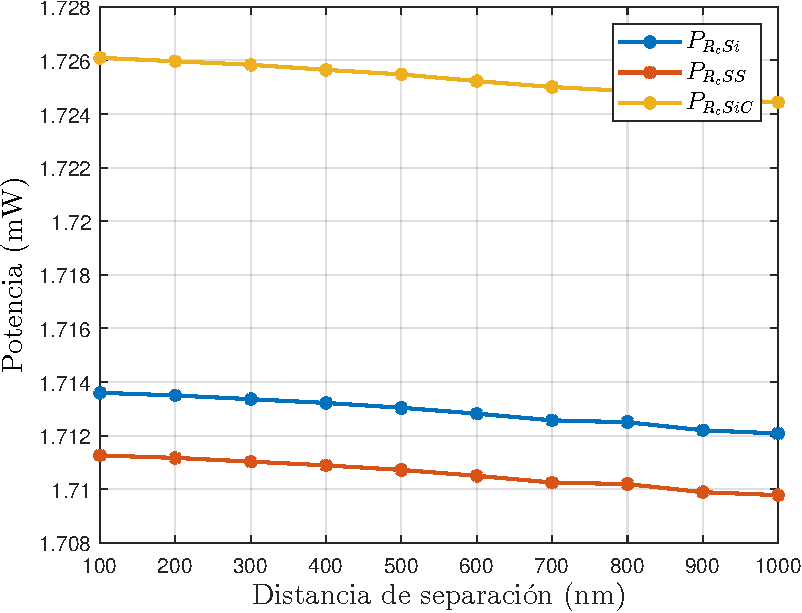
\includegraphics[width=\columnwidth]{Prc_XxSiGe}%
			\caption{}%
			\label{fig:prc_xxSi}%
	\end{subfigure}
	\hfill
	\begin{subfigure}[b]{0.48\textwidth}%
			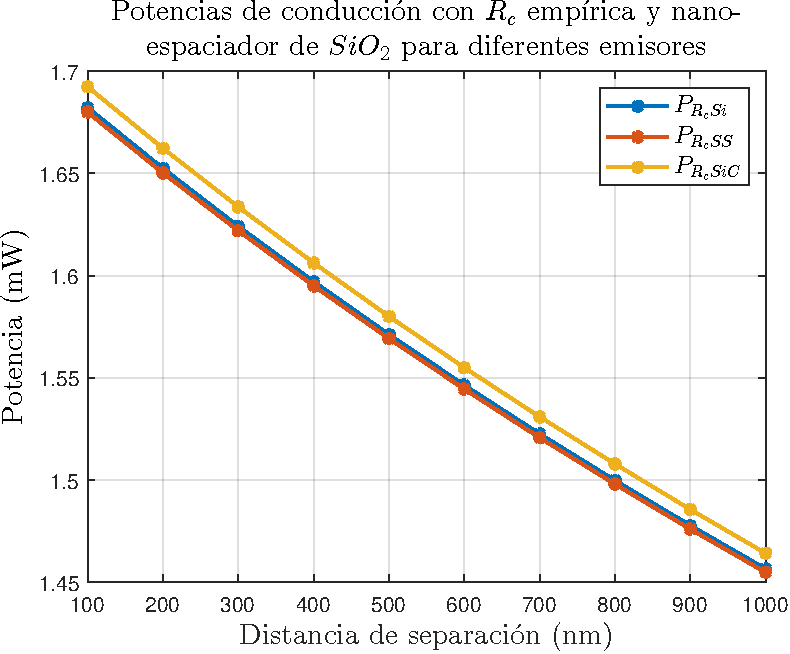
\includegraphics[width=\columnwidth]{Prc_XxSiO2Ge}%
			\caption{}%
			\label{fig:prc_xxSiO2}%
	\end{subfigure}
	\caption{Potencias transmitidas por conducci�n de unas nTPVs con emisores de $Si$, $SS$ y $SiC$ frente a las alturas de un solo nano-espaciador en nanometros para un nano-espaciador de $Si$ (\subref{fig:prc_xxSi}) y para un nano-espaciador de $SiO_2$ (\subref{fig:prc_xxSiO2}).}%
	\label{fig:prc_xxXX}%
\end{figure}
En segundo lugar, se observa como las curvas de las potencias de conducci�n no var�an tanto entre su valor m�ximo y valor m�nimo, siendo para el caso de las nTPVs con nano-espaciadores de $Si$ el que presenta la menor variaci�n de los dos, siendo esta menor de $0.002 \ mW$ (figura \ref{fig:prc_xxSi}), a diferencia de los nano-espaciadores de $SiO_2$ cuya variaci�n es menor a los $0.25 \ mW$ (figura \ref{fig:prc_xxSiO2}). Tambi�n se observa con mayor detalle como la diferencias de las resistencias t�rmicas de los materiales afecta al flujo de calor, aumentando con la disminuci�n de la resistencia t�rmica o aumento de la conductividad t�rmica, cuyos valores se mencionan en la secci�n \ref{sec:res_SiCSiO2Ge}.\\\\
En tercer lugar, las potencias de conducci�n son muy similares para ambos materiales de nano-espaciador con la altura de 100 nm porque la resistencia t�rmica de los nano-espaciadores disminuye considerablemente con la disminuci�n de la distancia, por ser proporcional a ella. Esto produce que la $R_c$ sea la principal resistencia t�rmica del sistema, por tal motivo, los valores de las potencias de conducci�n se asemejan a dicha altura del nano-espaciador.\\\\
Por �ltimo, se calculan las densidades de nano-espaciadores frente a las alturas de los nano-espaciadores para la nTPV de emisor de $SiC$ y nano-espaciadores de $Si$ (figura \ref{fig:prc_SiCSi}), y se compara con las densidades de la nTPV de emisor de $SiC$ pero nano-espaciadores de $SiO_2$ (figura \ref{fig:prc_SiCSiO2}). Se observa que existe una disminuci�n de las densidades para cada relaci�n de potencias y todas las alturas de los nano-espaciadores, siendo la m�s notable a los 1000 nm de altura y relaci�n de potencias de un orden de magnitud, pasando la densidad de ser $12 \ n^{\circ}esp/cm^2$ (figura \ref{fig:prc_SiCSiO2}) a ser $10 \ n^{\circ}esp/cm^2$ (figura \ref{fig:prc_SiCSi}). Esta poca variaci�n para dos materiales distintos de nano-esapciadores se d� porque para ambos casos la nTPV tiene una $R_c$ que es la resistencia t�rmica m�s significativa del sistema.
\begin{figure} [h]%
	\centering
	\begin{subfigure}[b]{0.48\textwidth}%
			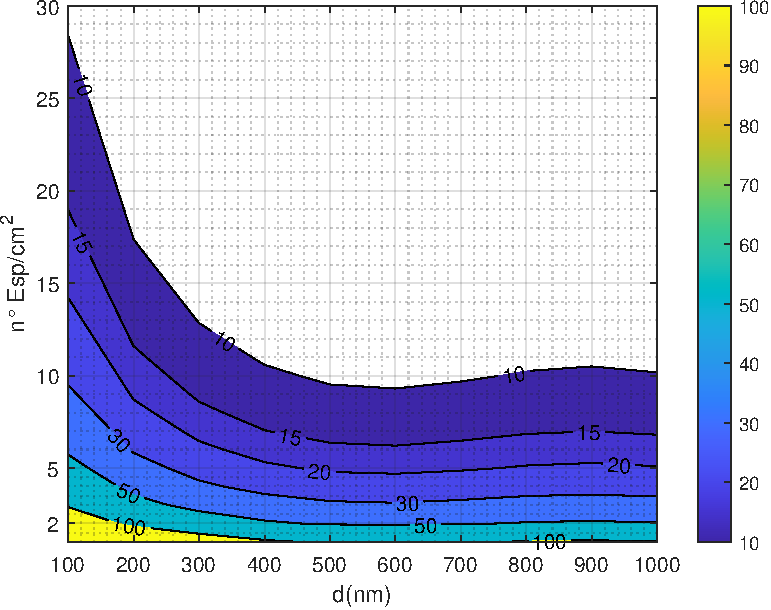
\includegraphics[width=\columnwidth]{rel_SiC}%
			\caption{}%
			\label{fig:prc_SiCSi}%
	\end{subfigure}
	\hfill
	\begin{subfigure}[b]{0.48\textwidth}%
			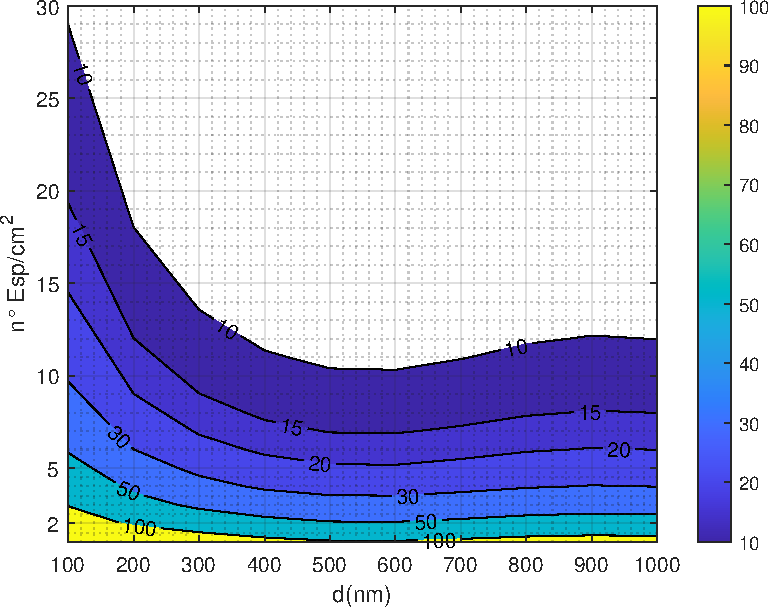
\includegraphics[width=\columnwidth]{SiC_Rc}%
			\caption{}%
			\label{fig:prc_SiCSiO2}%
	\end{subfigure}
	\caption{Densidades de nano-espaciadores ($n^{\circ}esp/cm^2$) frente a las alturas de los nano-espaciadores para todas las relaciones de la potencia de radiaci�n en el rango espectral de energ�as mayores e igual a 0.7 eV respecto a las potencias de conducci�n con $R_c$ (dependientes en la densidad de nano-espaciadores) mayores a 10 para nTPVs de nano-espaciadores de $Si$ (\subref{fig:prc_SiCSi}) y $SiO_2$(\subref{fig:prc_SiCSiO2}) . Donde las barras de colores laterales de cada gr�fica representan los colores asociados a cada uno de los valores de las relaciones de las potencias, con los contornos de las relaciones m�s significativas representadas en las gr�ficas.}%
	\label{fig:prc_SiCXX}%
\end{figure}
